\documentclass[tikz, border=1mm]{standalone}
\usepackage{tikz} 
\usetikzlibrary{arrows.meta}
\usepackage{pgfplots}

\begin{document}

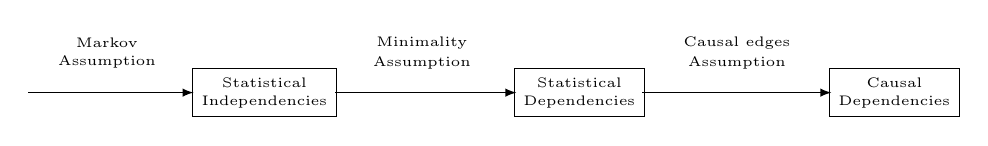
\begin{tikzpicture}
    % nodes
    \node at (-5,0.5) {\tiny{\shortstack{Markov \\ Assumption}}};
    \node at (-3,0) [rectangle,draw]  {\tiny{\shortstack{Statistical \\ Independencies}}};
    \node at (-1,0.5) {\tiny{\shortstack{Minimality \\ Assumption}}};
    \node at (1,0) [rectangle,draw]  {\tiny{\shortstack{Statistical \\ Dependencies}}};
    \node at (3,0.5) {\tiny{\shortstack{Causal edges \\ Assumption}}};
    \node at (5,0) [rectangle,draw]  {\tiny{\shortstack{Causal \\ Dependencies}}};
	% paths
    \draw[-{latex}](-6,0) to (-3.9,0);
    \draw[-{latex}](-2.1,0) to (0.2,0);
    \draw[-{latex}](1.8,0) to (4.2,0);
\end{tikzpicture}
  
\end{document}
